
% \subsection{Why apply causal models to synthetic data?}

This paper demonstrates how temporal causal models can be used as the basis of simulations that make it possible to optimize treatment policies in virtual experiments. We show the approach on data that has itself been generated by a simulation, so that we know the 'ground truth' causal relationships. Our ultimate goal is to optimize patient treatment protocols using simulations based on causal models derived from a combination of learning from patient data and incorporating domain knowledge.


% This paper demonstrates how simulated data can be used to build a predictor of disease progression that avoids limitations of retrospective observational data.  For purposes of demonstration we start with a canonical causal model from which we generate simulated data.  From this we attempt to reconstruct the model, much as would be done with actual data. By discovering what causal claims the data holds, we can use the model not only for prediction, but for testing treatment protocols that are justified by the causal nature of the model. Our approach consists of
% \begin{itemize}
%     \item Generating a simulation of a fictitious disease progression, along with its symptoms, drug regime, and outcomes;
%     \item Showing how current causal discovery tools can extract a model in the form of a causal network from the data with the help of an ``expert-in-the-loop, taking advantage of current medical knowledge;''
%     \item Relating how the causal nature of the resulting model explains the disease dynamics so that we can rediscover the optimal policy in the original simulation, avoiding limitations that arise with offline observational data. We show this by further simulations derived from the causal model.
% \end{itemize}

% With a method in hand to simulate clinical treatments as a basis to improve them from data, one could apply this to historical patient data and develop better treatments. 

% \subsection{Background on causal modelling}
% Making a causal claim is stronger than just quantifying the effect of modifying one variable on another.  A causal claim is a counterfactual  that can be explained in terms of  \emph{potential outcomes}. %\cite
% and is equivalent to the findings had one run a randomized experiment to determine the effect. A causal model may be represented by an a-cyclic directed network, which recently developed methods, such as~\cite{geffner2022} attempt to learn from sampled data. 

% Example - how lack of unrolling leads to confounding -- regression. 

% A causal explanation anchors the explanation to the actual phenomenon, that is in the real world.  We distinguish \emph{model explainability}---a property of the model---from a causal explanation that is a property of the world as revealed by the data. In our representation we express the causal effect by the probability $\Pr{effect}{do(cause)}$ using the conventional "do" notation [Pearl ]. 

% Synthea is an open source application created by XX in the U.S. NIH that simulates an extensive class of disease protocols.  These may be simulated over a presumed population that matches the demographics of a region, to simulate population health outcomes at the level of individual health records over the course of the individuals' lifetimes. In previous work the authors have demonstrated how to improve the veracity of the Synthea simulation by adjusting disease evolution probabilities within a protocol to match values learnt from existing patient clinical histories. 

% As for learning a patient model, conventional machine learning methods have been applied to build predictive models. For example, assuming a suitable reward function, one can directly learn appropriate policies from historical data using reinforcement learning.  This is similar but not as transparent as our approach where, figuratively, we split the modeling in two; first building a causal model from the data of the disease dynamics that can be inspected and validated against current medical knowledge, then applying the causal model to simulating the disease progression. Because it is causal, manipulating variables allow predictions of hypothetical future scenarios. [The point is that they explore parts of the space not seen in the history.]

% Explanation of the overall structure of/methods in the paper -- if short we can move to intro.
% \begin{figure}
%   \centering
%   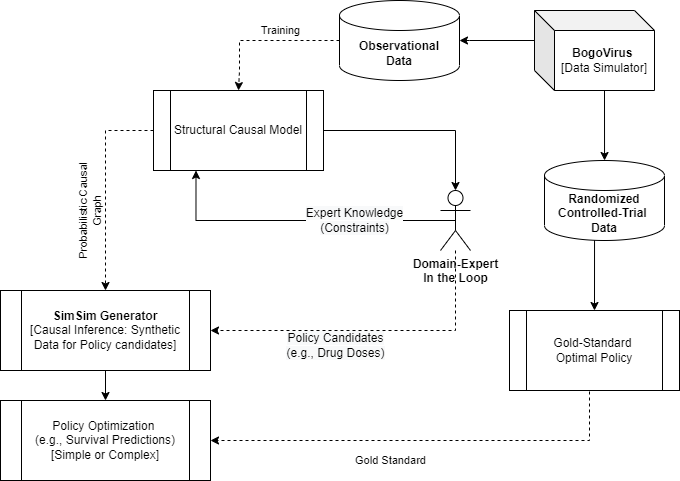
\includegraphics[width=0.7\linewidth]{figures/overview.png}
%   \caption{TBD: add explanation.}
%   \label{fig:pipeline_overview}
% \end{figure}